\documentclass[AMA,Times1COL]{WileyNJDv5} %STIX1COL,STIX2COL,STIXSMALL

%https://onlinelibrary.wiley.com/page/journal/15264025/homepage/forauthors.html
\articletype{Article Type}%

\received{Date Month Year}
\revised{Date Month Year}
\accepted{Date Month Year}
\journal{Journal}
\volume{00}
\copyyear{2025}
\startpage{1}

\raggedbottom

%
\begin{document}

\title{Determining Convergence for Bayesian Optimization}

\author[1]{Nicholas Grunloh}

\author[1]{Herbert Lee}

\authormark{Grunloh and Lee} %\textsc{et al.}}
\titlemark{Determining Convergence for Bayesian Optimization}

\address[1]{\orgdiv{Department of Statistical Sciences}, \orgname{University of California, Santa Cruz}, \orgaddress{\state{CA}, \country{USA}}}
%\address[2]{\orgdiv{Department Name}, \orgname{Institution Name}, \orgaddress{\state{State Name}, \country{Country Name}}}

\corres{Corresponding author Nicholas Grunloh. 110 McAllister Way, Santa Cruz, CA 95060  \email{grunloh@soe.ucsc.edu}}

%\presentaddress{This is sample for present address text this is sample for present address text.}

%\fundingInfo{Text}
%\JELinfo{ejlje}

\abstract[Abstract]{
Bayesian optimization routines may have theoretical convergence results, but
determining whether a run has converged in practice can be a subjective task.
This paper provides a framework inspired by statistical process control for
monitoring an optimization run for convergence. An Exponentially Weighted
Moving Average chart is adapted for automated convergence analysis.
}

\keywords{Derivative-free Optimization, Computer Simulation, Emulator, Expected Improvement}

\jnlcitation{\cname{%
\author{Grunloh N} and
\author{Lee H}}.
\ctitle{Determining Convergence for Bayesian Optimization.} 
%\cjournal{\it J Comput Phys.} \cvol{2021;00(00):1--18}.
}


\maketitle

\renewcommand\thefootnote{}
\footnotetext{\textbf{Abbreviations:} ELAI, Expected Log-Normal Approximation of Improvement; EWMA, Exponentially Weighted Moving Average.}

\renewcommand\thefootnote{\fnsymbol{footnote}}
\setcounter{footnote}{1}


%
%
\section{Introduction}
%
%

%
Bayesian optimization aims to find a global optimum of a complex function that 
may not be analytically tractable, and where derivative information may not be 
readily available \citep{mockus:1989,brochu:2010}. A common application is for 
computer simulation experiments \cite{gramacy:2020}. Because each function 
evaluation may be expensive, one wants to terminate the optimization algorithm 
as early as possible. However for complex simulators, the response surface may 
be ill-behaved and optimization routines can easily become trapped in a local 
mode, so one needs to run the optimization sufficiently long to achieve a 
robust solution. So far there has been little work on assessing convergence for 
Bayesian optimization. In this paper, we provide an automated method for 
determining convergence of surrogate model-based optimization by bringing in
elements of statistical process control.


%Black-box derivative-free optimization has a wide variety of applications,
%especially in the realm of computer simulations
%\citep{KoldLewiTorc2003,gramacy2014}.  When dealing with computationally
%expensive computer models, a key question is that of convergence of the
%optimization. Because each function evaluation is expensive, one wants to
%terminate the optimization as early as possible.  However for complex
%simulators, the response surface may be ill-behaved and optimization routines
%can easily become trapped in a local mode, so one needs to run the optimization
%sufficiently long to achieve a robust solution. So far there have been no
%reliable solutions for assessing convergence of surrogate model optimization.
%In this paper, we provide an automated method for determining convergence of
%Gaussian process surrogate model optimization by bringing in elements of
%Statistical Process Control.

%
%
%
%Our motivating example is a hydrology application, the Lockwood pump-and-treat
%problem \citep{lockCite}, discussed in more detail in
%Section~\ref{sec:lockwood}, wherein contamination in the groundwater near the
%Yellowstone River is remediated via a set of treatment wells. The goal is to
%minimize the cost of running the wells while ensuring that no contamination
%enters the river. The contamination constraint results in a complicated
%boundary that is unknown in advance and requires evaluation of the simulator.
%Finding the global constrained minimum is a difficult problem where it is easy
%for optimization routines to temporarily get stuck in a local minimum.  Without
%knowing the answer in advance, how does one know when to terminate the
%optimization algorithm? 
%
%
%

%
Among the wide variety of Bayesian optimization approaches, we focus on those
that are based on a statistical surrogate model, such as a Gaussian process
\citep{santnerBook}. We further focus on approaches based on Expected
Improvement (EI) \citep{gBook}, although our methods are generalizable for other
acquisition functions.

%
%

%%\clearpage
%%however; as a means of assessing convergence GP surrogate
%%{\color{red}Literature cite} recommends considering the EI as a convergence 
%%criterion for surrogate model optimization; as of yet, little work has been 
%%done to describe what convergence of these algorithms actually looks like in 
%%the context of the EI criterion.
%%, but it has not yet been established if there is some threshold EI value 
%%that is sufficient claim that there exists 
%%in many different; of many other numerical optimization routines; that have 
%%been designed specifically to exhibit such behavior upon convergence  This 
%%use of EI as a convergence criterion is analogous to other standard 
%%convergence identification methods in numerical optimization (e.g., the 
%%vanishing step sizes of a Newton-Raphson algorithm).%However, applying this 
%%same threshold strategy to the convergence of surrogate model optimization has 
%%not yet been adequately justified.
%%, derived from the predictive distribution of the underling GP model; behavior
%\cite{taddyOpt} considers the use of the improvement distribution for 
%identifying global convergence; stating its value for use in applied 
%optimization. The basic idea behind the use of improvement in identifying 
%convergence is that convergence should occur when the surrogate model produces 
%low expectations for discovering a new optimum; that is to say, globally small 
%EI values should be associated with convergence of the algorithm. Thus a 
%simplistic stopping rule might first define some lower EI threshold, then 
%claim convergence upon the first instance of an EI value falling below this 
%threshold, as seen in \cite{windExample}. 
%In fact, this use of EI ignores the 
%nature of the EI criterion as a random variable, and oversimplifies the 
%stochastic nature of convergence in this setting. Thus it is no surprise that 
%this treatment of the EI criterion can result in an inconsistent stopping rule 
%as demonstrated in \mbox{Figure (\ref{introFig}).}

%
There have been a few hints in the literature that monitoring EI directly could
be used to assess convergence \citep{jonesEIOpt}. \cite{taddyOpt} considers the
use of the improvement distribution for identifying global convergence. The
basic idea is that convergence should occur when the surrogate model produces
low expectations for discovering a new optimum; that is to say, globally small
EI values should be associated with convergence of the algorithm. Thus a
simplistic stopping rule might first define some lower EI threshold, then claim
convergence upon the first instance of an EI value falling below this threshold,
as seen in \cite{windExample}. This use of EI as a convergence criterion is
analogous to other standard convergence identification methods in numerical
optimization (e.g., the vanishing step sizes of a Newton-Raphson algorithm).
However, applying this same threshold strategy to the convergence of Bayesian
optimization has not yet been adequately justified. In fact, this use of EI
ignores the nature of the EI criterion as a random variable, and oversimplifies
the stochastic nature of convergence in this setting. Thus it is no surprise
that this treatment of the EI criterion can result in an inconsistent stopping
rule as demonstrated in \mbox{Figure (\ref{introFig}).}

%\clearpage
%
%
\begin{figure}[htb]
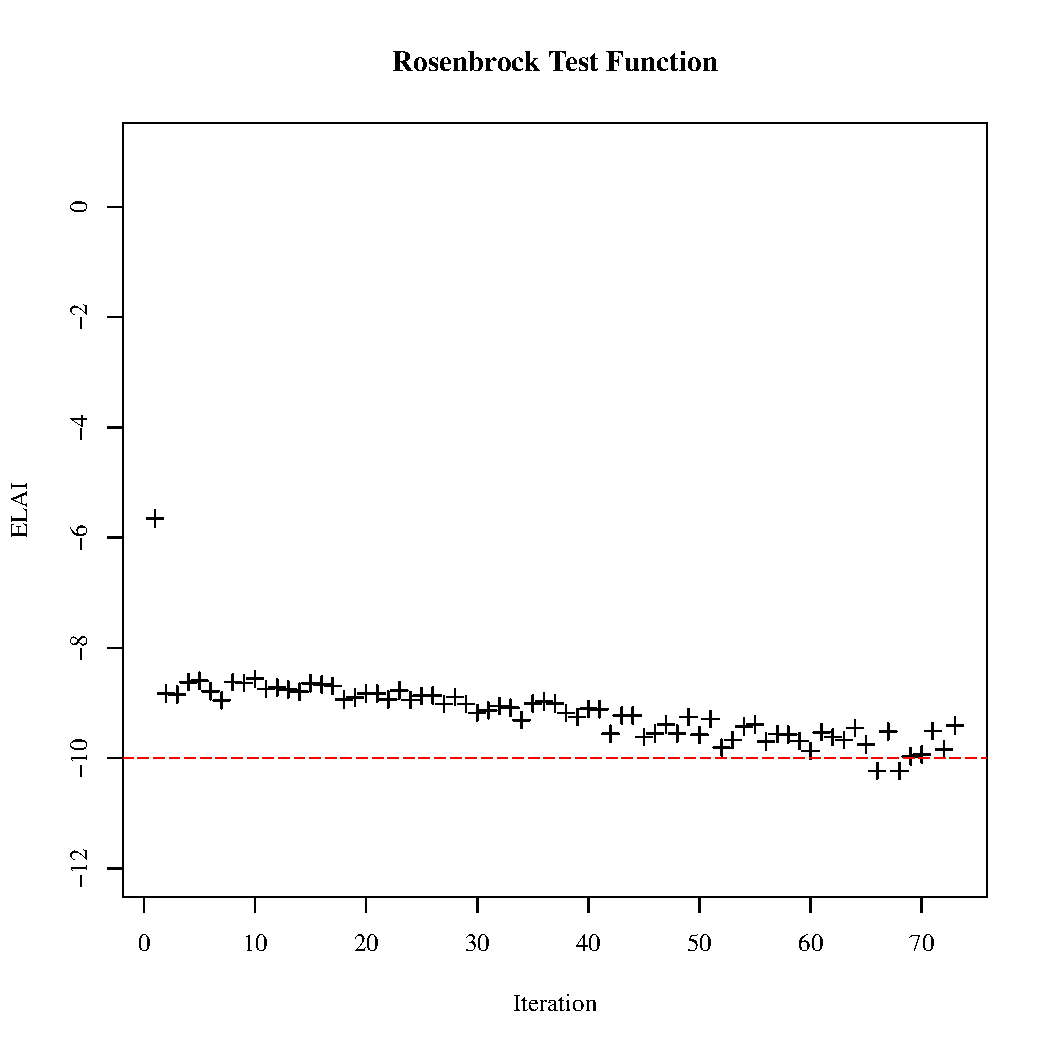
\includegraphics[width=0.32\textwidth]{./figures/introChartRoseEasyEasyAxis.pdf}
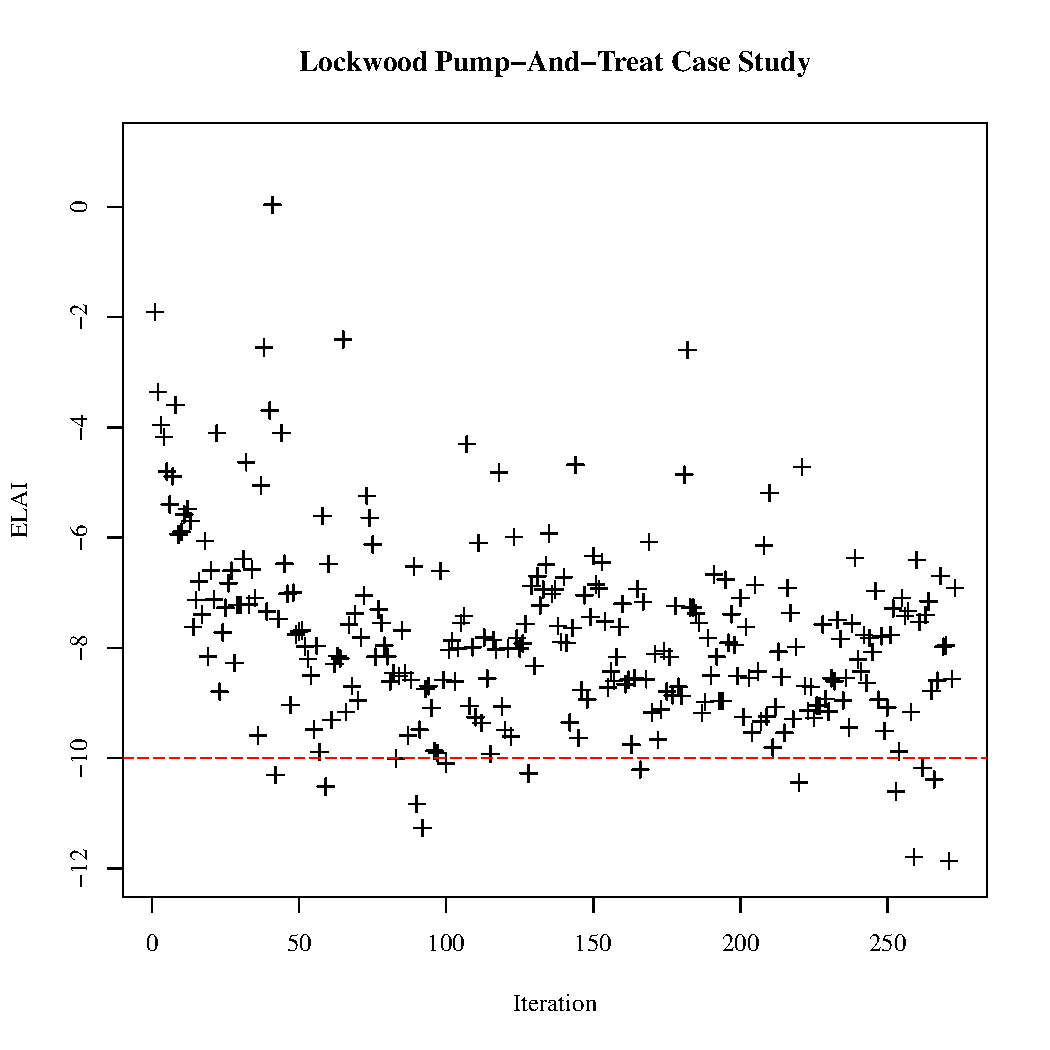
\includegraphics[width=0.32\textwidth]{./figures/introChartLock6Three20000Axis.pdf}
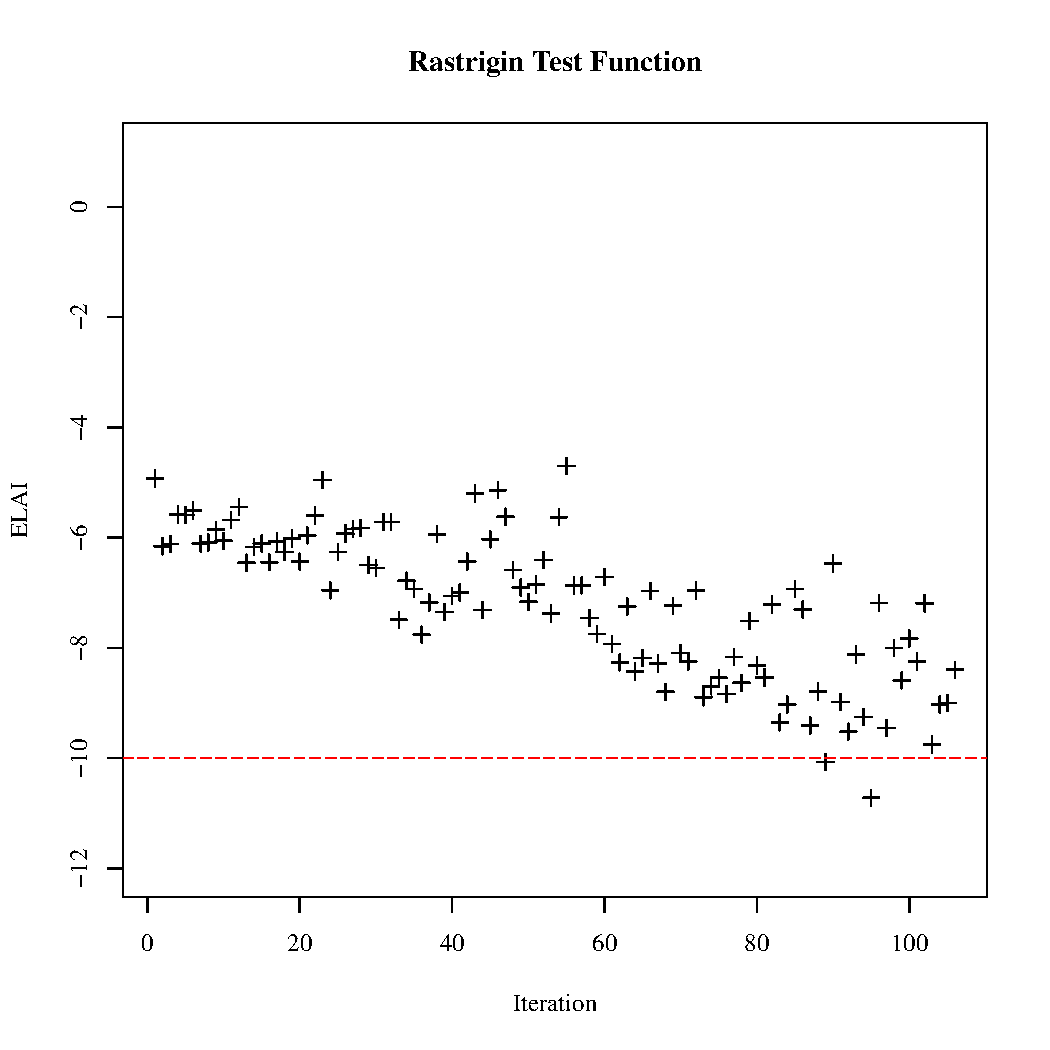
\includegraphics[width=0.32\textwidth]{./figures/introChartRastHardAxis.pdf}
\caption{
%
Three Expected Log-normal Approximation to the Improvement series (more details 
in Section~\ref{sec:examples}) plotted alongside an example convergence 
threshold value shown as a dashed line at -10.
}
\label{introFig}
\end{figure}
%
%

%%of the series value; of the values; shows; non-negative
%Because EI is strictly positive but decreasingly small,
%we find it more productive to work on the log scale, using a log-normal
%approximation to the improvement distribution to generate a more appropriate convergence criterion, as described in more
%detail in Section~3.2.
%%
%Figure~(\ref{introFig}) represents three series of the Expected
%Log-normal Approximation to the Improvement (ELAI) convergence criterion values from three
%different optimization problems that will be demonstrated later in
%this paper, where it will be shown that convergence is established near
%the end of each of these series.
%%as generated by 
%These three series demonstrate various ELAI convergence behaviors, and
%illustrate the difficulty in assessing convergence.  
%asymptotic properties of the; in more detail; improve
%In each panel the y-axis represents a monotone transformation of the basic EI criterion {\color{red}(i.e. ELI)} so as to 
%benefit the asymptotic behavior of the improvement criterion's distribution, to be discussed further in Section {\color{red}XX}
%, additionally as the algorithm proceeds, several improvements of the objective function are discovered while ELI values 
%repeatedly fall below the convergence threshold. 
%, all while the optimization routine continues to find several improved values of the objective function.

%of the series value; of the values; shows; non-negative
Because EI is strictly positive but decreasingly small, we find it more
productive to work on the log scale, using a log-normal approximation to the
improvement distribution to generate a more appropriate convergence criterion,
as described in Section~3.2. Figure~(\ref{introFig}) represents three series of
the Expected Log-normal Approximation to the Improvement (ELAI) values from
three different optimization problems. We will demonstrate later in this paper
that convergence is established near the end of each of these series. These
three series demonstrate the kind of diversity observed among various ELAI
convergence behaviors, and illustrate the difficulty in assessing convergence.
In the left-most panel, optimization of the Rosenbrock test function results in
a well-behaved series of ELAI values, demonstrating a case in which the simple
threshold stopping rule can accurately identify convergence.  However the center
panel (the Lockwood problem described in Section~4.3) demonstrates a failure of
the threshold stopping rule, as this ELAI series contains much more variance,
and thus small ELAI values are observed quite regularly. In the Lockwood example
a simple threshold stopping rule could falsely claim convergence within the
first 50 iterations of the algorithm. The large variability in ELAI values with
occasional large values indicates that the optimization routine sometimes
briefly settles into a local minimum but is still exploring and is not yet
convinced that it has found a global minimum. This optimization run appears to
have converged only after the larger ELAI values stop appearing and the
variability has decreased. Thus one might ask if a decrease in variability, or
small variability, is a necessary condition for convergence. The right-most
panel (the Rastrigin test function) shows a case where convergence occurs by
meeting the threshold level, but where variability has increased, demonstrating
that a decrease in variability is not a necessary condition.

%
%

%
Since the Improvement function is itself random, attempting to set a lower
threshold bound on the EI, without consideration of the underlying EI
distribution through time, over-simplifies the dynamics of convergence in this
setting. Instead, we propose taking the perspective of Statistical Process
Control (SPC), where a stochastic series is monitored for consistency of the
distribution of the most recently observed values. In the next section, we
review the surrogate model approach and the use of EI for
optimization. In Section~\ref{sec:convergence}, we discuss our inspiration from
SPC and how we construct our convergence chart. Section~\ref{sec:examples}
provides synthetic and real examples, and then we provide some conclusions in
the final section.

%\clearpage
%
%
\section{Bayesian Optimization via Expected Improvement}
\label{sec:gp}
%
%
























%%
%\clearpage
%\newgeometry{ margin=1in, top=0.6in, footskip=0.4in }
%\singlespacing
%\bibliographystyle{jasa}
%\bibliographystyle{apalike}
%\bibliographystlye{natbib}
%\bibliographystyle{NJDapacite}
\bibliography{spcCite}






%%
%{\color{red}
%
%
%\section{First level head}\label{sec1}
%
%Please lay out your article using the section headings and the given body text
%is dummy text for layout purpose.  Lorem ipsum dolor sit amet, consectetuer
%adipiscing elit \cite{Hirt1974}. Ut purus elit, vestibulum ut, placerat ac,
%adipiscing vitae, felis. Curabitur dictum gravida mauris. Nam arcu libero,
%nonummy eget, consectetuer id, vulputate a, magna. Donec vehicula augue eu
%neque. Pellentesque habitant morbi tristique senectus et netus et malesuada
%fames ac turpis egestas.  Mauris ut leo. Cras viverra metus rhoncus sem. Nulla
%et lectus vestibulum urna fringilla ultrices. Phasellus eu tellus sit amet
%tortor gravida placerat. Integer sapien est, iaculis in, pretium quis, viverra
%ac, nunc. Praesent eget sem vel leo ultrices bibendum. Aenean faucibus. Morbi
%dolor nulla, malesuada eu, pulvinar at, mollis ac, nulla. Curabitur auctor
%semper nulla. Donec varius orci eget risus. Duis nibh mi, congue eu, accumsan
%eleifend, sagittis quis, diam.  Duis eget orci sit amet orci dignissim rutrum.
%
%
%\section{Another first level head}\label{sec2}
%
%Nulla malesuada porttitor diam. Donec felis erat, congue non, volutpat at,
%tincidunt tristique, libero. Vivamus viverra fermentum felis. Donec nonummy
%pellentesque ante. Phasellus adipiscing semper elit. Proin fermentum massa ac
%quam. Sed diam turpis, molestie vitae, placerat a, molestie nec, leo
%\cite{Liska2010}. Maecenas lacinia. Nam ipsum ligula, eleifend at, accumsan nec,
%suscipit a, ipsum. Morbi blandit ligula feugiat magna. Nunc eleifend consequat
%lorem. Sed lacinia nulla vitae enim. Pellentesque tincidunt purus vel magna.
%Integer non enim. Praesent euismod nunc eu purus. Donec bibendum quam in tellus.
%Nullam cursus pulvinar lectus. Donec et mi. Nam vulputate metus eu enim.
%Vestibulum pellentesque felis eu massa. Example for bibliography citation
%\cite{Taylor1937}, text \cite{Knupp1999,Kamm2000} inserted in text for your
%reference.
%
%Quisque ullamcorper placerat ipsum. Cras nibh \cite{Kucharik2003,Blanchard2015}.
%Morbi vel justo vitae lacus tincidunt ultrices. Lorem ipsum dolor sit amet,
%consectetuer adipiscing elit. In hac habitasse platea dictumst. Integer tempus
%convallis augue. Etiam facilisis.  Nunc elementum fermentum wisi. Aenean
%placerat. Ut imperdiet, enim sed gravida sollicitudin, felis odio placerat quam,
%ac pulvinar elit purus eget enim. Nunc vitae tortor. Proin tempus nibh sit amet
%nisl. Vivamus quis tortor vitae risus porta vehicula.
%
%Fusce mauris. Vestibulum luctus nibh at lectus. Sed bibendum, nulla a faucibus
%semper, leo velit ultricies tellus, ac venenatis arcu wisi vel nisl. Vestibulum
%diam. (Figure \ref{fig1} and \ref{fig2}) Aliquam pellentesque, augue quis
%sagittis posuere, turpis lacus congues quam, in hendrerit risus eros eget felis.
%Maecenas eget erat in sapien mattis porttitor. Vestibulum porttitor. Nulla
%facilisi. Sed a turpis eu lacus commodo facilisis. Morbi fringilla, wisi in
%dignissim interdum, justo lectus sagittis dui, et vehicula libero dui cursus
%dui. Mauris tempor ligula sed lacus. Duis cursus enim ut augue. Cras ac magna.
%Cras nulla.  Nulla egestas. Curabitur a leo. Quisque egestas wisi eget nunc. Nam
%feugiat lacus vel est. Curabitur consectetuer.
%
%
%\begin{figure*}[t]
%\centerline{
\includegraphics[width=\textwidth,height=9pc,draft]{empty}}
%\caption{This is the sample figure caption.\label{fig1}} \end{figure*}
%
%Suspendisse vel felis. Ut lorem lorem, interdum eu, tincidunt sit amet, laoreet
%vitae, arcu. Aenean faucibus pede eu ante. Praesent enim elit, rutrum at,
%molestie non, nonummy vel, nisl. Ut lectus eros, malesuada sit amet, fermentum
%eu, sodales cursus, magna. Donec eu purus. Quisque vehicula, urna sed ultricies
%auctor, pede lorem egestas dui, et convallis elit erat sed nulla. Donec luctus.
%Curabitur et nunc. Aliquam dolor odio, commodo pretium, ultricies non, pharetra
%in, velit. Integer arcu est, nonummy in, fermentum faucibus, egestas vel, odio.
%\begin{align*} s(nT_{s}) &= s(t)\times \sum\limits_{n=0}^{N-1} \delta (t-nT_{s})
%\xleftrightarrow{\mathrm{DFT}}  S \left(\frac{m}{NT_{s}}\right) \nonumber\\[3pt]
%&= \frac{1}{N} \sum\limits_{n=0}^{N-1} \sum\limits_{k=-N/2}^{N/2-1} s_{k}
%e^{\mathrm{j}2\pi k\Delta fnT_{s}} e^{-j\frac{2\pi}{N}mn} \end{align*}
%
%
%Sed commodo posuere pede. Mauris ut est. Ut quis purus. Sed ac odio. Sed
%vehicula hendrerit sem. Duis non odio. Morbi ut dui. Sed accumsan risus eget
%odio. In hac habitasse platea dictumst. Pellentesque non elit. Fusce sed justo
%eu urna porta tincidunt. Mauris felis odio, sollicitudin sed, volutpat a, ornare
%ac, erat. Morbi quis dolor.  Donec pellentesque, erat ac sagittis semper, nunc
%dui lobortis purus, quis congue purus metus ultricies tellus. Proin et quam.
%Class aptent taciti sociosqu ad litora torquent per conubia nostra, per inceptos
%hymenaeos. Praesent sapien turpis, fermentum vel, eleifend faucibus, vehicula
%eu, lacus.
%
%\begin{figure*}
%\centerline{
\includegraphics[width=342pt,height=9pc,draft]{empty}} \caption{This
%is the sample figure caption.\label{fig2}} \end{figure*}
%
%\subsection{Second level head}
%
%Pellentesque habitant morbi tristique senectus et netus et malesuada fames ac
%turpis egestas. Donec odio elit, dictum in, hendrerit sit amet, egestas sed,
%leo. Praesent feugiat sapien aliquet odio. Integer vitae justo. Aliquam
%vestibulum fringilla lorem. Sed neque lectus, consectetuer at, consectetuer sed,
%eleifend ac, lectus. Nulla facilisi. Pellentesque eget lectus. Proin eu metus.
%Sed porttitor. In hac habitasse platea dictumst. Suspendisse eu lectus. Ut mi
%mi, lacinia sit amet, placerat et, mollis vitae, dui. Sed ante tellus, tristique
%ut, iaculis eu, malesuada ac, dui. Mauris nibh leo, facilisis non, adipiscing
%quis, ultrices a, dui.
%
%Morbi luctus, wisi viverra faucibus pretium, nibh est placerat odio, nec commodo
%wisi enim eget quam. Quisque libero justo, consectetuer a, feugiat vitae,
%porttitor eu, libero. Suspendisse sed mauris vitae elit sollicitudin malesuada.
%
%Maecenas ultricies eros sit amet ante. Ut venenatis velit. Maecenas sed mi eget
%dui varius euismod. Phasellus aliquet volutpat odio. Vestibulum ante ipsum
%primis in faucibus orci luctus et ultrices posuere cubilia Curae; Pellentesque
%sit amet pede ac sem eleifend consectetuer. Nullam elementum, urna vel imperdiet
%sodales, elit ipsum pharetra ligula, ac pretium ante justo a nulla. Curabitur
%tristique arcu eu metus. Vestibulum lectus. Proin mauris. Proin eu nunc eu urna
%hendrerit faucibus. Aliquam auctor, pede consequat laoreet varius, eros tellus
%scelerisque quam, pellentesque hendrerit ipsum dolor sed augue. Nulla nec lacus.
%
%\begin{quote} This is an example \cite{Burton2013,Berndt2011,Kucharik2012} for
%quote text. This is an example for quote text. This is an example for quote
%text. This is an example for quote text \cite{Breil2015}. This is an example for
%quote text. This is an example for quote text. This is an example for quote
%text. This is an example for quote text. This is an example for quote text. This
%is an example for quote text \cite{Barth1997}. This is an example for quote
%text. This is an example for quote text. This is an example for quote text.
%\end{quote}
%
%\section{Example for another first level head}\label{sec3}
%
%\subsection{Example for another second level head}
%
%Suspendisse vitae elit. Aliquam arcu neque, ornare in, ullamcorper quis, commodo
%eu, libero. Fusce sagittis erat at erat tristique mollis. Maecenas sapien
%libero, molestie et, lobortis in, sodales eget, dui. Morbi ultrices rutrum
%lorem.  Nam elementum ullamcorper leo. Morbi dui. Aliquam sagittis. Nunc
%placerat. Pellentesque tristique sodales est.  Maecenas imperdiet lacinia velit.
%Cras non urna. Morbi eros pede, suscipit ac, varius vel, egestas non, eros.
%Praesent malesuada, diam id pretium elementum, eros sem dictum tortor, vel
%consectetuer odio sem sed wisi.
%
%Sed feugiat. Cum sociis natoque penatibus et magnis dis parturient montes,
%nascetur ridiculus mus. Ut pellentesque augue sed urna. Vestibulum diam eros,
%fringilla et, consectetuer eu, nonummy id, sapien. Nullam at lectus. In sagittis
%ultrices mauris. Curabitur malesuada erat sit amet massa. Fusce blandit. Aliquam
%erat volutpat. Aliquam euismod.  Aenean vel lectus. Nunc imperdiet justo nec
%dolor.
%
%\subsection{Second level head}
%
%Etiam euismod. Fusce facilisis lacinia dui. Suspendisse potenti. In mi erat,
%cursus id, nonummy sed, ullamcorper eget, sapien. Praesent pretium, magna in
%eleifend egestas, pede pede pretium lorem, quis consectetuer tortor sapien
%facilisis magna. Mauris quis magna varius nulla scelerisque imperdiet. Aliquam
%non quam. Aliquam porttitor quam a lacus. Praesent vel arcu ut tortor cursus
%volutpat. In vitae pede quis diam bibendum placerat. Fusce elementum convallis
%neque. Sed dolor orci, scelerisque ac, dapibus nec, ultricies ut, mi. Duis nec
%dui quis leo sagittis commodo.
%
%
%\subsubsection{Third level head}
%
%Aliquam lectus. Vivamus leo. Quisque ornare tellus ullamcorper nulla. Mauris
%porttitor pharetra tortor. Sed fringilla justo sed mauris. Mauris tellus. Sed
%non leo. Nullam elementum, magna in cursus sodales, augue est scelerisque
%sapien, venenatis congue nulla arcu et pede. Ut suscipit enim vel sapien. Donec
%congue. Maecenas urna mi, suscipit in, placerat ut, vestibulum ut, massa. Fusce
%ultrices nulla et nisl.
%
%\paragraph{Fourth level head}
%
%Sed feugiat. Cum sociis natoque penatibus et magnis dis parturient montes,
%nascetur ridiculus mus. Ut pellentesque augue sed urna. Vestibulum diam eros,
%fringilla et, consectetuer eu, nonummy id, sapien. Nullam at lectus. In sagittis
%ultrices mauris. Curabitur malesuada erat sit amet massa. Fusce blandit. Aliquam
%erat volutpat. Aliquam euismod.  Aenean vel lectus. Nunc imperdiet justo nec
%dolor.
%
%Etiam euismod. Fusce facilisis lacinia dui. Suspendisse potenti. In mi erat,
%cursus id, nonummy sed, ullamcorper eget, sapien. Praesent pretium, magna in
%eleifend egestas, pede pede pretium lorem, quis consectetuer tortor sapien
%facilisis magna. Mauris quis magna varius nulla scelerisque imperdiet. Aliquam
%non quam. Aliquam porttitor quam a lacus. Praesent vel arcu ut tortor cursus
%volutpat. In vitae pede quis diam bibendum placerat. Fusce elementum convallis
%neque. Sed dolor orci, scelerisque ac, dapibus nec, ultricies ut, mi. Duis nec
%dui quis leo sagittis commodo.
%
%\subparagraph{Fifth level head.}
%
%Aliquam lectus. Vivamus leo. Quisque ornare tellus ullamcorper nulla. Mauris
%porttitor pharetra tortor. Sed fringilla justo sed mauris. Mauris tellus. Sed
%non leo. Nullam elementum, magna in cursus sodales, augue est scelerisque
%sapien, venenatis congue nulla arcu et pede. Ut suscipit enim vel sapien. Donec
%congue. Maecenas urna mi, suscipit in, placerat ut, vestibulum ut, massa. Fusce
%ultrices nulla et nisl.
%
%Etiam ac leo a risus tristique nonummy. Donec dignissim tincidunt nulla.
%Vestibulum rhoncus molestie odio. Sed lobortis, justo et pretium lobortis,
%mauris turpis condimentum augue, nec ultricies nibh arcu pretium enim. Nunc
%purus neque, placerat id, imperdiet sed, pellentesque nec, nisl. Vestibulum
%imperdiet neque non sem accumsan laoreet.  In hac habitasse platea dictumst.
%Etiam condimentum facilisis libero. Suspendisse in elit quis nisl aliquam
%dapibus.  Pellentesque auctor sapien. Sed egestas sapien nec lectus.
%Pellentesque vel dui vel neque bibendum viverra. Aliquam porttitor nisl nec
%pede. Proin mattis libero vel turpis. Donec rutrum mauris et libero. Proin
%euismod porta felis.  Nam lobortis, metus quis elementum commodo, nunc lectus
%elementum mauris, eget vulputate ligula tellus eu neque.  Vivamus eu dolor.
%
%Nulla in ipsum. Praesent eros nulla, congue vitae, euismod ut, commodo a, wisi.
%Pellentesque habitant morbi tristique senectus et netus et malesuada fames ac
%turpis egestas. Aenean nonummy magna non leo. Sed felis erat, ullamcorper in,
%dictum non, ultricies ut, lectus. Proin vel arcu a odio lobortis euismod.
%Vestibulum ante ipsum primis in faucibus orci luctus et ultrices posuere cubilia
%Curae; Proin ut est. Aliquam odio. Pellentesque massa turpis, cursus eu, euismod
%nec, tempor congue, nulla. Duis viverra gravida mauris. Cras tincidunt.
%Curabitur eros ligula, varius ut, pulvinar in, cursus faucibus, augue (Box~1).
%
%
%Etiam ac leo a risus tristique nonummy. Donec dignissim tincidunt nulla.
%Vestibulum rhoncus molestie odio. Sed lobortis, justo et pretium lobortis,
%mauris turpis condimentum augue, nec ultricies nibh arcu pretium enim. Nunc
%purus neque, placerat id, imperdiet sed, pellentesque nec, nisl. Vestibulum
%imperdiet neque non sem accumsan laoreet.  In hac habitasse platea dictumst.
%Etiam condimentum facilisis libero. Suspendisse in elit quis nisl aliquam
%dapibus.  Pellentesque auctor sapien. Sed egestas sapien nec lectus.
%Pellentesque vel dui vel neque bibendum viverra. Aliquam porttitor nisl nec
%pede. Proin mattis libero vel turpis. Donec rutrum mauris et libero. Proin
%euismod porta felis.  Nam lobortis, metus quis elementum commodo, nunc lectus
%elementum mauris, eget vulputate ligula tellus eu neque.  Vivamus eu dolor.
%
%\begin{boxwithhead} {BOX 1\quad This is sample for Box head and text} {\noindent
%This is sample for boxtext this is sample for boxtext this is sample for boxtext
%this is sample for boxtext this is sample for boxtext this is sample for boxtext
%this is sample for boxtext this is sample for boxtext this is sample for boxtext
%this is sample for boxtext this is sample for boxtext this is sample for boxtext
%this is sample for boxtext this is sample for boxtext this is sample for boxtext
%this is sample for boxtext this is sample for boxtext this is sample for boxtext
%this is sample for boxtext this is sample for boxtext this is sample for boxtext
%this is sample for boxtext this is sample for boxtext this is sample for boxtext
%this is sample for boxtext this is sample for boxtext this is sample for boxtext
%this is sample for boxtext this is sample for boxtext this is sample for boxtext
%this is sample for boxtext this is sample for boxtext this is sample for boxtext
%this is sample for boxtext this is sample for boxtext this is sample for boxtext
%this is sample for boxtext this is sample for boxtext this is sample for boxtext
%this is sample for boxtext this is sample for boxtext this is sample for boxtext
%this is sample for boxtext this is sample for boxtext this is sample for boxtext
%this is sample for boxtext this is sample for boxtext. This is sample for
%boxtext this is sample for boxtext this is sample for boxtext this is sample for
%boxtext this is sample for boxtext this is sample for boxtext this is sample for
%boxtext this is sample for boxtext this is sample for boxtext this is sample for
%boxtext this is sample for boxtext this is sample for boxtext this is sample for
%boxtext this is sample for boxtext this is sample for boxtext this is sample for
%boxtext this is sample for boxtext this is sample for boxtext this is sample for
%boxtext this is sample for boxtext this is sample for boxtext this is sample for
%boxtext this is sample for boxtext this is sample for boxtext this is sample for
%boxtext this is sample for boxtext this is sample for boxtext this is sample for
%boxtext this is sample for boxtext this is sample for boxtext this is sample for
%boxtext this is sample for boxtext this is sample for boxtext this is sample for
%boxtext this is sample for boxtext this is sample for boxtext this is sample for
%boxtext this is sample for boxtext this is sample for boxtext this is sample for
%boxtext this is sample for boxtext this is sample for boxtext this is sample for
%boxtext this is sample for boxtext this is sample for boxtext this is sample for
%boxtext this is sample for boxtext.} \end{boxwithhead}
%
%
%
%
%%\begin{center} \begin{table*}[!h]% \caption{This is sample table
%%caption.\label{tab1}} \begin{tabular*}{\textwidth}{@{\extracolsep\fill}lllll@{}}
%%\toprule &\multicolumn{2}{@{}l}{\textbf{Spanned heading$^{\tnote{\bf a}}$}} &
%%\multicolumn{2}{@{}l}{\textbf{Spanned heading$^{\tnote{\bf b}}$}}
%%\\\cmidrule{2-3}\cmidrule{4-5} \textbf{Col1 head} & \textbf{Col2 head}  &
%%\textbf{Col3 head}  & {\textbf{Col4 head}}  & \textbf{Col5 head}   \\ \midrule
%%col1 text & col2 text  & col3 text  & 12.34  & col5 text\tnote{1}   \\ col1 text
%%& col2 text  & col3 text  & \hphantom{0}1.62  & col5 text\tnote{2}   \\ col1
%%text & col2 text  & col3 text  & 51.809  & col5 text   \\ \bottomrule
%%\end{tabular*} \begin{tablenotes}%%[341pt] \item[$^{\rm a}$] Example for a first
%%table footnote.  \item[$^{\rm b}$] Example for a second table footnote.  \item
%%{\it Source}: Example for table source text.  \end{tablenotes} \end{table*}
%%\end{center}
%
%Curabitur tellus magna, porttitor a, commodo a, commodo in, tortor. Donec
%interdum (Table~\ref{tab1}).  Praesent scelerisque. Maecenas posuere sodales
%odio. Vivamus metus lacus, varius quis, imperdiet quis, rhoncus a, turpis. Etiam
%ligula arcu, elementum a, venenatis quis, sollicitudin sed, metus. Donec nunc
%pede, tincidunt in, venenatis vitae, faucibus vel, nibh. Pellentesque wisi.
%Nullam malesuada. Morbi ut tellus ut pede tincidunt porta. Lorem ipsum dolor sit
%amet, consectetuer adipiscing elit. Etiam congue neque id dolor.
%
%
%Donec et nisl at wisi luctus bibendum. Nam interdum tellus ac libero. Sed sem
%justo, laoreet vitae, fringilla at, adipiscing ut, nibh. Maecenas non sem quis
%tortor eleifend fermentum. Etiam id tortor ac mauris porta vulputate.  Integer
%porta neque vitae massa. Maecenas tempus libero a libero posuere dictum.
%Vestibulum ante ipsum primis in faucibus orci luctus et ultrices posuere cubilia
%Curae; Aenean quis mauris sed elit commodo placerat. Class aptent taciti
%sociosqu ad litora torquent per conubia nostra, per inceptos hymenaeos. Vivamus
%rhoncus tincidunt libero.  Etiam elementum pretium justo. Vivamus est. Morbi a
%tellus eget pede tristique commodo. Nulla nisl. Vestibulum sed nisl eu sapien
%cursus rutrum.
%
%%\begin{boxtext}% {\noindent This is sample for boxtext this is sample for
%%boxtext this is sample for boxtext this is sample for boxtext this is sample for
%%boxtext this is sample for boxtext this is sample for boxtext this is sample for
%%boxtext this is sample for boxtext this is sample for boxtext this is sample for
%%boxtext this is sample for boxtext this is sample for boxtext this is sample for
%%boxtext this is sample for boxtext this is sample for boxtext.} \end{boxtext}
%
%Nulla non mauris vitae wisi posuere convallis. Sed eu nulla nec eros scelerisque
%pharetra. Nullam varius. Etiam dignissim elementum metus. Vestibulum faucibus,
%metus sit amet mattis rhoncus, sapien dui laoreet odio, nec ultricies nibh augue
%a enim. Fusce in ligula. Quisque at magna et nulla commodo consequat. Proin
%accumsan imperdiet sem.  Nunc porta. Donec feugiat mi at justo. Phasellus
%facilisis ipsum quis ante. In ac elit eget ipsum pharetra faucibus.  Maecenas
%viverra nulla in massa (Table~\ref{tab2}).
%
%Nulla in ipsum. Praesent eros nulla, congue vitae, euismod ut, commodo a, wisi.
%Pellentesque habitant morbi tristique senectus et netus et malesuada fames ac
%turpis egestas. Aenean nonummy magna non leo. Sed felis erat, ullamcorper in,
%dictum non, ultricies ut, lectus. Proin vel arcu a odio lobortis euismod.
%Vestibulum ante ipsum primis
%
%
%
%Fusce mauris. Vestibulum luctus nibh at lectus. Sed bibendum, nulla a faucibus
%semper, leo velit ultricies tellus, ac venenatis arcu wisi vel nisl. Vestibulum
%diam. Aliquam pellentesque, augue quis sagittis posuere, turpis lacus congue
%quam, in hendrerit risus eros eget felis. Maecenas eget erat in sapien mattis
%porttitor. Vestibulum porttitor. Nulla facilisi. Sed a turpis eu lacus commodo
%facilisis. Morbi fringilla, wisi in dignissim interdum, justo lectus sagittis
%dui, et vehicula libero dui cursus dui. Mauris tempor ligula sed lacus. Duis
%cursus enim ut augue. Cras ac magna. Cras nulla.  Nulla egestas. Curabitur a
%leo. Quisque egestas wisi eget nunc. Nam feugiat lacus vel est. Curabitur
%consectetuer.
%
%
%%\begin{table*}[!t]% \centering % \caption{This is sample table
%%caption.\label{tab2}}%
%%\begin{tabular*}{\textwidth}{@{\extracolsep\fill}lllll@{\extracolsep\fill}}
%%\toprule \textbf{Col1 head} & \textbf{Col2 head}  & \textbf{Col3 head}  &
%%\textbf{Col4 head}  & \textbf{Col5 head} \\ \midrule col1 text & col2 text  &
%%col3 text  & col4 text  & col5 text\tnote{$^\dagger$}   \\ col1 text & col2 text
%%& col3 text  & col4 text  & col5 text   \\ col1 text & col2 text  & col3 text  &
%%col4 text  & col5 text\tnote{$^\ddagger$}   \\ \bottomrule \end{tabular*}
%%\begin{tablenotes} \item[$^\dagger$] Example for a first table footnote.
%%\item[$^\ddagger$] Example for a second table footnote.  \item {\it Source}:
%%Example for table source text.  \end{tablenotes} \end{table*}
%
%Below is the example \cite{Liska2010,Kucharik2003,Blanchard2015} for bulleted
%list. Below is the example for bulleted list. Below is the example for bulleted
%list. Below is the example for bulleted list. Below is the example for bulleted
%list. Below is the example for bulleted list\footnote{This is an example for
%footnote.}: \begin{itemize} \item bulleted list entry sample bulleted list entry
%\cite{Lauritzen2011}, sample list entry text.  \item bulleted list entry sample
%bulleted list entry. bulleted list entry sample bulleted list entry. bulleted
%list entry sample bulleted list entry.  \item bulleted list entry sample
%bulleted list entry \cite{Klima2017}, bulleted list entry sample bulleted list
%entry \cite{Dukowicz2000}, sample list entry text.  bulleted list entry sample
%bulleted list entry.  \item sample list entry text. sample list entry text.
%\end{itemize}
%
%Suspendisse vel felis. Ut lorem lorem, interdum eu, tincidunt sit amet, laoreet
%vitae, arcu. Aenean faucibus pede eu ante. Praesent enim elit, rutrum at,
%molestie non, nonummy vel, nisl. Ut lectus eros, malesuada sit amet, fermentum
%eu, sodales cursus, magna. Donec eu purus. Quisque vehicula, urna sed ultricies
%auctor, pede lorem egestas dui, et convallis elit erat sed nulla. Donec luctus.
%Curabitur et nunc. Aliquam dolor odio, commodo pretium, ultricies non, pharetra
%in, velit. Integer arcu est, nonummy in, fermentum faucibus, egestas vel, odio.
%
%Sed commodo posuere pede. Mauris ut est. Ut quis purus. Sed ac odio. Sed
%vehicula hendrerit sem. Duis non odio. Morbi ut dui. Sed accumsan risus eget
%odio. In hac habitasse platea dictumst. Pellentesque non elit. Fusce sed justo
%eu urna porta tincidunt. Mauris felis odio, sollicitudin sed, volutpat a, ornare
%ac, erat. Morbi quis dolor. Donec pellentesque, erat ac sagittis semper, nunc
%dui lobortis purus, quis congue purus metus ultricies tellus. Proin et quam.
%Class aptent taciti sociosqu ad litora torquent per conubia nostra, per inceptos
%hymenaeos. Praesent sapien turpis, fermentum vel, eleifend faucibus, vehicula
%eu, lacus.
%
%
%Pellentesque non elit. Fusce sed justo eu urna porta tincidunt. Mauris felis
%odio, sollicitudin sed, volutpat a, ornare ac, erat. Morbi quis dolor. Donec
%pellentesque, erat ac sagittis semper, nunc dui lobortis purus, quis congue
%purus metus ultricies tellus. Proin et quam. Below is the example for
%description list. Below is the example for description list. Below is the
%example for description list. Below is the example for description list. Below
%is the example for description list. Below is the sample for description list.
%Below is the example for description list. Below is the example for description
%list. Below is the example for description list. Below is the example for
%description list. Below is the example for description list:\vskip12pt
%
%
%\noindent\textbf{Description sample:} \begin{description} \item[first entry]
%description text, description text \cite{Kucharik2011,Kucharik2014,Loubere2005}.
%description text, description text, description text, description text,
%description text.  \item[second long entry] description text, description text,
%description text, description text, description text, description text,
%description text.  \item[third entry] description text, description text,
%description text, description text, description text.  \item[fourth entry]
%description text, description text.  \end{description}
%
%
%\noindent\textbf{Numbered list items sample:}
%
%\begin{enumerate}[1.] \item First level numbered list entry, sample numbered
%list entry.
%
%\item First numbered list entry, sample numbered list entry. Numbered list entry
%\cite{Caramana1998}, sample numbered list entry. Numbered list entry, sample
%numbered list entry.
%
%\begin{enumerate}[a.] \item Second level alpabetical list entry. Second level
%alpabetical list entry. Second level alpabetical list entry \cite{Hoch2009}.
%Second level alpabetical list entry.
%
%\item Second level alpabetical list entry. Second level alpabetical list entry
%\cite{Shashkov1996,Knupp1999,Knupp1999}.
%
%\begin{enumerate}[i.] \item Third level lowercase roman numeral list entry.
%Third level lowercase roman numeral list entry. Third level lowercase roman
%numeral list entry.
%
%\item Third level lowercase roman numeral list entry. Third level lowercase
%roman numeral list entry. \cite{Kamm2000} \end{enumerate}
%
%\item Second level alpabetical list entry. Second level alpabetical list entry
%\cite{Taylor1937}.  \end{enumerate}
%
%\item First level numbered list entry, sample numbered list entry. Numbered list
%entry, sample numbered list entry. Numbered list entry.
%
%\item Another first level numbered list entry, sample numbered list entry.
%Numbered list entry, sample numbered list entry. Numbered list entry.
%\end{enumerate}
%
%\noindent\textbf{un-numbered list items sample:}
%
%\begin{enumerate}[] \item Sample unnumberd list text.  \item Sample unnumberd
%list text.  \item sample unnumberd list text.  \item Sample unnumberd list text.
%\end{enumerate}
%
%\section{Examples for enunciations}\label{sec4}
%
%\begin{theorem}\label{thm1} Example theorem text. Example theorem text. Example
%theorem text. Example theorem text. Example theorem text. Example theorem text.
%Example theorem text. Example theorem text. Example theorem text. Example
%theorem text. Example theorem text. Example theorem text. Example theorem text.
%Example theorem text. Example theorem text. Example theorem text. Example
%theorem text. Example theorem text. Example theorem text. Example theorem text.
%Example theorem text. Example theorem text. Example theorem text. Example
%theorem text. Example theorem text.  \end{theorem}
%
%Quisque ullamcorper placerat ipsum. Cras nibh. Morbi vel justo vitae lacus
%tincidunt ultrices. Lorem ipsum dolor sit amet, consectetuer adipiscing elit. In
%hac habitasse platea dictumst. Integer tempus convallis augue. Etiam facilisis.
%Nunc elementum fermentum wisi. Aenean placerat. Ut imperdiet, enim sed gravida
%sollicitudin, felis odio placerat quam, ac pulvinar elit purus eget enim. Nunc
%vitae tortor. Proin tempus nibh sit amet nisl. Vivamus quis tortor vitae risus
%porta vehicula.
%
%Fusce mauris. Vestibulum luctus nibh at lectus. Sed bibendum, nulla a faucibus
%semper, leo velit ultricies tellus, ac venenatis arcu wisi vel nisl. Vestibulum
%diam. Aliquam pellentesque, augue quis sagittis posuere, turpis lacus congue
%quam, in hendrerit risus eros eget felis. Maecenas eget erat in sapien mattis
%porttitor. Vestibulum porttitor. Nulla facilisi. Sed a turpis eu lacus commodo
%facilisis. Morbi fringilla, wisi in dignissim interdum, justo lectus sagittis
%dui, et vehicula libero dui cursus dui. Mauris tempor ligula sed lacus. Duis
%cursus enim ut augue. Cras ac magna. Cras nulla.  Nulla egestas. Curabitur a
%leo. Quisque egestas wisi eget nunc. Nam feugiat lacus vel est. Curabitur
%consectetuer.
%
%\begin{proposition} Example proposition text. Example proposition text. Example
%proposition text. Example proposition text. Example proposition text. Example
%proposition text. Example proposition text. Example proposition text. Example
%proposition text. Example proposition text. Example proposition text. Example
%proposition text. Example proposition text. Example proposition text. Example
%proposition text. Example proposition text.  \end{proposition}
%
%Nulla malesuada porttitor diam. Donec felis erat, congue non, volutpat at,
%tincidunt tristique, libero. Vivamus viverra fermentum felis. Donec nonummy
%pellentesque ante. Phasellus adipiscing semper elit. Proin fermentum massa ac
%quam. Sed diam turpis, molestie vitae, placerat a, molestie nec, leo. Maecenas
%lacinia. Nam ipsum ligula, eleifend at, accumsan nec, suscipit a, ipsum. Morbi
%blandit ligula feugiat magna. Nunc eleifend consequat lorem. Sed lacinia nulla
%vitae enim. Pellentesque tincidunt purus vel magna. Integer non enim. Praesent
%euismod nunc eu purus. Donec bibendum quam in tellus. Nullam cursus pulvinar
%lectus. Donec et mi. Nam vulputate metus eu enim. Vestibulum pellentesque felis
%eu massa.
%
%Quisque ullamcorper placerat ipsum. Cras nibh. Morbi vel justo vitae lacus
%tincidunt ultrices. Lorem ipsum dolor sit amet, consectetuer adipiscing elit. In
%hac habitasse platea dictumst. Integer tempus convallis augue. Etiam facilisis.
%Nunc elementum fermentum wisi. Aenean placerat. Ut imperdiet, enim sed gravida
%sollicitudin, felis odio placerat quam, ac pulvinar elit purus eget enim. Nunc
%vitae tortor. Proin tempus nibh sit amet nisl. Vivamus quis tortor vitae risus
%porta vehicula.
%
%\begin{definition} Example definition text. Example definition text. Example
%definition text. Example definition text. Example definition text. Example
%definition text. Example definition text. Example definition text. Example
%definition text. Example definition text. Example definition text.
%\end{definition}
%
%Sed commodo posuere pede. Mauris ut est. Ut quis purus. Sed ac odio. Sed
%vehicula hendrerit sem. Duis non odio. Morbi ut dui. Sed accumsan risus eget
%odio. In hac habitasse platea dictumst. Pellentesque non elit. Fusce sed justo
%eu urna porta tincidunt. Mauris felis odio, sollicitudin sed, volutpat a, ornare
%ac, erat. Morbi quis dolor.  Donec pellentesque, erat ac sagittis semper, nunc
%dui lobortis purus, quis congue purus metus ultricies tellus. Proin et quam.
%Class aptent taciti sociosqu ad litora torquent per conubia nostra, per inceptos
%hymenaeos. Praesent sapien turpis, fermentum vel, eleifend faucibus, vehicula
%eu, lacus.
%
%Pellentesque habitant morbi tristique senectus et netus et malesuada fames ac
%turpis egestas. Donec odio elit, dictum in, hendrerit sit amet, egestas sed,
%leo. Praesent feugiat sapien aliquet odio. Integer vitae justo. Aliquam
%vestibulum fringilla lorem. Sed neque lectus, consectetuer at, consectetuer sed,
%eleifend ac, lectus. Nulla facilisi.  Pellentesque eget lectus. Proin eu metus.
%Sed porttitor. In hac habitasse platea dictumst. Suspendisse eu lectus. Ut mi
%mi, lacinia sit amet, placerat et, mollis vitae, dui. Sed ante tellus, tristique
%ut, iaculis eu, malesuada ac, dui.  Mauris nibh leo, facilisis non, adipiscing
%quis, ultrices a, dui.
%
%\begin{proof} Example for proof text. Example for proof text. Example for proof
%text. Example for proof text. Example for proof text. Example for proof text.
%Example for proof text. Example for proof text. Example for proof text. Example
%for proof text.  \end{proof}
%
%Nam dui ligula, fringilla a, euismod sodales, sollicitudin vel, wisi. Morbi
%auctor lorem non justo. Nam lacus libero, pretium at, lobortis vitae, ultricies
%et, tellus. Donec aliquet, tortor sed accumsan bibendum, erat ligula aliquet
%magna, vitae ornare odio metus a mi. Morbi ac orci et nisl hendrerit mollis.
%Suspendisse ut massa. Cras nec ante. Pellentesque a nulla. Cum sociis natoque
%penatibus et magnis dis parturient montes, nascetur ridiculus mus. Aliquam
%tincidunt urna. Nulla ullamcorper vestibulum turpis. Pellentesque cursus luctus
%mauris.
%
%Nulla malesuada porttitor diam. Donec felis erat, congue non, volutpat at,
%tincidunt tristique, libero. Vivamus viverra fermentum felis. Donec nonummy
%pellentesque ante. Phasellus adipiscing semper elit. Proin fermentum massa ac
%quam. Sed diam turpis, molestie vitae, placerat a, molestie nec, leo. Maecenas
%lacinia. Nam ipsum ligula, eleifend at, accumsan nec, suscipit a, ipsum. Morbi
%blandit ligula feugiat magna. Nunc eleifend consequat lorem. Sed lacinia nulla
%vitae enim. Pellentesque tincidunt purus vel magna. Integer non enim. Praesent
%euismod nunc eu purus. Donec bibendum quam in tellus. Nullam cursus pulvinar
%lectus. Donec et mi. Nam vulputate metus eu enim. Vestibulum pellentesque felis
%eu massa.
%
%\begin{proof}[Proof of Theorem~{\rm\ref{thm1}}] Example for proof text. Example
%for proof text. Example for proof text. Example for proof text. Example for
%proof text. Example for proof text. Example for proof text. Example for proof
%text. Example for proof text. Example for proof text.  \end{proof}
%
%%\begin{sidewaystable}%[h] \def\d{\hphantom{0}} \caption{Sideways table caption.
%%For decimal alignment refer column 4 to 9 in tabular* preamble.\label{tab3}}%
%%\begin{tabular*}{\textheight}{@{\extracolsep\fill}lllllllll@{\extracolsep\fill}}%
%%\toprule & \textbf{Col2 head} & \textbf{Col3 head} &
%%\multicolumn{1}{l}{\textbf{10}} &\multicolumn{1}{l}{\textbf{20}}
%%&\multicolumn{1}{l}{\textbf{30}} &\multicolumn{1}{l}{\textbf{10}}
%%&\multicolumn{1}{l}{\textbf{20}} &\multicolumn{1}{l}{\textbf{30}} \\ \midrule
%%&col2 text &col3 text &\d0.7568&\d1.0530&\d1.2642&\d0.9919&\d1.3541&\d1.6108 \\
%%&          &col2 text &12.5701 &19.6603&25.6809&18.0689&28.4865&37.3011 \\ 3
%%&col2 text & col3 text &\d0.7426&\d1.0393&\d1.2507&\d0.9095&\d1.2524&\d1.4958 \\
%%&          &col3 text &12.8008&19.9620&26.0324&16.6347&26.0843&34.0765 \\ & col2
%%text& col3 text &\d0.7285&\d1.0257&\d1.2374&\d0.8195&\d1.1407&\d1.3694* \\ &
%%& col3 text &13.0360&20.2690&26.3895&15.0812&23.4932&30.6060\tnote{$\dagger$}
%%\\ \bottomrule \end{tabular*} \begin{tablenotes}%%[\textheight] \item[*] First
%%sideways table footnote. Sideways table footnote. Sideways table footnote.
%%Sideways table footnote.  \item[$^\dagger$] Second sideways table footnote.
%%Sideways table footnote. Sideways table footnote. Sideways table footnote.
%%\end{tablenotes} \end{sidewaystable}
%
%Etiam euismod. Fusce facilisis lacinia dui. Suspendisse potenti. In mi erat,
%cursus id, nonummy sed, ullamcorper eget, sapien. Praesent pretium, magna in
%eleifend egestas, pede pede pretium lorem, quis consectetuer tortor sapien
%facilisis magna. Mauris quis magna varius nulla scelerisque imperdiet. Aliquam
%non quam. Aliquam porttitor quam a lacus. Praesent vel arcu ut tortor cursus
%volutpat. In vitae pede quis diam bibendum placerat. Fusce elementum convallis
%neque. Sed dolor orci, scelerisque ac, dapibus nec, ultricies ut, mi. Duis nec
%dui quis leo sagittis commodo.  Aliquam lectus. Vivamus leo. Quisque ornare
%tellus ullamcorper nulla. Mauris porttitor pharetra tortor. Sed fringilla justo
%sed mauris. Mauris tellus. Sed non leo. Nullam elementum, magna in cursus
%sodales, augue est scelerisque sapien, venenatis congue nulla arcu et pede. Ut
%suscipit enim vel sapien. Donec congue. Maecenas urna mi, suscipit in, placerat
%ut, vestibulum ut, massa. Fusce ultrices nulla et nisl (Table~\ref{tab3}).
%
%Pellentesque habitant morbi tristique senectus et netus et malesuada fames ac
%turpis egestas. Donec odio elit, dictum in, hendrerit sit amet, egestas sed,
%leo. Praesent feugiat sapien aliquet odio. Integer vitae justo. Aliquam
%vestibulum fringilla lorem. Sed neque lectus, consectetuer at, consectetuer sed,
%eleifend ac, lectus. Nulla facilisi (Figure~\ref{fig3}).  Pellentesque eget
%lectus. Proin eu metus. Sed porttitor. In hac habitasse platea dictumst.
%Suspendisse eu lectus. Ut Curabitur tellus magna, porttitor a, commodo a,
%commodo in, tortor. Donec interdum. Praesent scelerisque. Mae- cenas posuere
%sodales odio. Vivamus metus lacus, varius quis, imperdiet quis, rhoncus a,
%turpis. Etiam ligula arcu, elementum a, venenatis quis, sollicitudin sed, metus.
%Donec nunc pede, tincidunt in, venenatis vitae, faucibus vel.
%
%
%
%\begin{sidewaysfigure}
%\centerline{
\includegraphics[width=542pt,height=9pc,draft]{empty}}
%\caption{Sideways figure caption. Sideways figure caption. Sideways figure
%caption. Sideways figure caption. Sideways figure caption. Sideways figure
%caption.\label{fig3}} \end{sidewaysfigure}
%
%Pellentesque wisi. \cite{Kucharik2012} Nullam malesuada. Morbi ut tellus ut pede
%tincidunt porta. Lorem ipsum dolor sit amet, consectetuer adipiscing elit. Etiam
%congue neque id dolor.
%
%
%\begin{algorithm} \caption{\enskip Pseudocode for our algorithm}\label{alg1}
%\begin{algorithmic} \For each frame \For water particles $f_{i}$ \State compute
%fluid flow \cite{Hirt1974} \State compute fluid--solid interaction
%\cite{Benson1992} \State apply adhesion and surface tension \cite{Margolin2003}
%\EndFor \For solid particles $s_{i}$ \For neighboring water particles $f_{j}$
%\State compute virtual water film \\(see Section~\ref{sec3}) \EndFor \EndFor
%\For solid particles $s_{i}$ \For neighboring water particles $f_{j}$ \State
%compute growth direction vector \\(see Section~\ref{sec2}) \EndFor \EndFor \For
%solid particles $s_{i}$ \For neighboring water particles $f_{j}$ \State compute
%$F_{\theta}$ (see Section~\ref{sec1}) \State compute $CE(s_{i},f_{j})$ \\(see
%Section~\ref{sec3}) \If $CE(b_{i}, f_{j})$ $>$ glaze threshold \State $j$th
%water particle's phase $\Leftarrow$ ICE \EndIf \If $CE(c_{i}, f_{j})$ $>$ icicle
%threshold \State $j$th water particle's phase $\Leftarrow$ ICE \EndIf \EndFor
%\EndFor \EndFor \end{algorithmic} \end{algorithm}
%
%Donec et nisl at wisi luctus bibendum. Nam interdum tellus ac libero. Sed sem
%justo, laoreet vitae, fringilla at, adipiscing ut, nibh. Maecenas non sem quis
%tortor eleifend fermentum. Etiam id tortor ac mauris porta vulputate.  Integer
%porta neque vitae massa \cite{Hirt1974,Benson1992}.  Maecenas tempus libero a
%libero posuere dictum. Vestibulum ante ipsum primis in faucibus orci luctus et
%ultrices posuere cubilia Curae; Aenean quis mauris sed elit commodo placerat.
%Class aptent taciti sociosqu ad litora torquent per conubia nostra, per inceptos
%hymenaeos. Vivamus rhoncus tincidunt libero.  Etiam elementum pretium justo.
%Vivamus est. Morbi a tellus eget pede tristique commodo \cite{Benson1992}. Nulla
%nisl. Vestibulum sed nisl eu sapien cursus rutrum.
%
%Pellentesque wisi. Nullam malesuada. Morbi ut tellus ut pede tincidunt porta.
%Lorem ipsum dolor sit amet, consectetuer adipiscing elit. Etiam congue neque id
%dolor.
%
%Donec et nisl at wisi luctus bibendum. Nam interdum tellus ac libero. Sed sem
%justo, laoreet vitae, fringilla at, adipiscing ut, nibh. Integer porta neque
%vitae massa. Maecenas tempus libero a libero posuere dictum. Vestibulum ante
%ipsum primis in faucibus orci luctus et ultrices posuere cubilia Curae; Aenean
%quis mauris sed elit commodo placerat.  Maecenas non sem quis tortor eleifend
%fermentum. Etiam id tortor ac mauris porta vulputate.  Integer porta neque vitae
%massa. Maecenas tempus libero a libero posuere dictum. Vestibulum ante ipsum
%primis in faucibus orci luctus et ultrices posuere cubilia Curae; Aenean quis
%mauris sed elit commodo placerat. Class aptent taciti sociosqu ad litora
%torquent per conubia nostra, per inceptos hymenaeos. Vivamus rhoncus tincidunt
%libero.  Etiam elementum pretium justo. Vivamus est. Morbi a tellus eget pede
%tristique commodo. Nulla nisl. Vestibulum sed nisl eu sapien cursus rutrum.
%\begin{align}\label{eq23} \|\tilde{X}(k)\|^2
%&=\frac{\left\|\sum\limits_{i=1}^{p}\tilde{Y}_i(k)+\sum\limits_{j=1}^{q}\tilde{Z}_j(k)
%\right\|^2}{(p+q)^2} \nonumber\\ &
%\leq\frac{\sum\limits_{i=1}^{p}\left\|\tilde{Y}_i(k)\right\|^2+\sum\limits_{j=1}^{q}\left\|\tilde{Z}_j(k)\right\|^2
%}{p+q}.  \end{align}
%
%Sed feugiat. Cum sociis natoque penatibus et magnis dis parturient montes,
%nascetur ridiculus mus. Ut pellentesque augue sed urna. Vestibulum diam eros,
%fringilla et, consectetuer eu, nonummy id, sapien. Nullam at lectus. In sagittis
%ultrices mauris. Curabitur malesuada erat sit amet massa. Fusce blandit. Aliquam
%erat volutpat. Aliquam euismod.  Aenean vel lectus. Nunc imperdiet justo nec
%dolor.
%
%Etiam euismod. Fusce facilisis lacinia dui. Suspendisse potenti. In mi erat,
%cursus id, nonummy sed, ullamcorper eget, sapien. Praesent pretium, magna in
%eleifend egestas, pede pede pretium lorem, quis consectetuer tortor sapien
%facilisis magna. Mauris quis magna varius nulla scelerisque imperdiet. Aliquam
%non quam. Aliquam porttitor quam a lacus. Praesent vel arcu ut tortor cursus
%volutpat. In vitae pede quis diam bibendum placerat. Fusce elementum convallis
%neque. Sed dolor orci, scelerisque ac, dapibus nec, ultricies ut, mi. Duis nec
%dui quis leo sagittis commodo.  \begin{align}\label{eq24} \|\tilde{X}(k)\|^2
%&=\frac{\left\|\sum\limits_{i=1}^{p}\tilde{Y}_i(k)+\sum\limits_{j=1}^{q}\tilde{Z}_j(k)
%\right\|^2}{(p+q)^2}\nonumber\\ &
%\leq\frac{\sum\limits_{i=1}^{p}\left\|\tilde{Y}_i(k)\right\|^2+\sum\limits_{j=1}^{q}\left\|\tilde{Z}_j(k)\right\|^2
%}{p+q}.  \end{align}
%
%Aliquam lectus. Vivamus leo. Quisque ornare tellus ullamcorper nulla. Mauris
%porttitor pharetra tortor. Sed fringilla justo sed mauris. Mauris tellus. Sed
%non leo. Nullam elementum, magna in cursus sodales, augue est scelerisque
%sapien, venenatis congue nulla arcu et pede. Ut suscipit enim vel sapien. Donec
%congue. Maecenas urna mi, suscipit in, placerat ut, vestibulum ut, massa. Fusce
%ultrices nulla et nisl.
%
%Etiam ac leo a risus tristique nonummy. Donec dignissim tincidunt nulla.
%Vestibulum rhoncus molestie odio. Sed lobortis, justo et pretium lobortis,
%mauris turpis condimentum augue, nec ultricies nibh arcu pretium enim. Nunc
%purus neque, placerat id, imperdiet sed, pellentesque nec, nisl. Vestibulum
%imperdiet neque non sem accumsan laoreet.  In hac habitasse platea dictumst.
%Etiam condimentum facilisis libero. Suspendisse in elit quis nisl aliquam
%dapibus.  Pellentesque auctor sapien. Sed egestas sapien nec lectus.
%Pellentesque vel dui vel neque bibendum viverra. Aliquam porttitor nisl nec
%pede. Proin mattis libero vel turpis. Donec rutrum mauris et libero. Proin
%euismod porta felis.  Nam lobortis, metus quis elementum commodo, nunc lectus
%elementum mauris, eget vulputate ligula tellus eu neque.  Vivamus eu dolor.
%
%
%
%
%\section{Conclusions}\label{sec5}
%
%Lorem ipsum dolor sit amet, consectetuer adipiscing elit. Ut purus elit,
%vestibulum ut, placerat ac, adipiscing vitae, felis. Curabitur dictum gravida
%mauris. Nam arcu libero, nonummy eget, consectetuer id, vulputate a, magna.
%Donec vehicula augue eu neque. Pellentesque habitant morbi tristique senectus et
%netus et malesuada fames ac turpis egestas.  Mauris ut leo. Cras viverra metus
%rhoncus sem. Nulla et lectus vestibulum urna fringilla ultrices. Phasellus eu
%tellus sit amet tortor gravida placerat. Integer sapien est, iaculis in, pretium
%quis, viverra ac, nunc. Praesent eget sem vel leo ultrices bibendum. Aenean
%faucibus. Morbi dolor nulla, malesuada eu, pulvinar at, mollis ac, nulla.
%Curabitur auctor semper nulla. Donec varius orci eget risus. Duis nibh mi,
%congue eu, accumsan eleifend, sagittis quis, diam.  Duis eget orci sit amet orci
%dignissim rutrum.
%
%Nam dui ligula, fringilla a, euismod sodales, sollicitudin vel, wisi. Morbi
%auctor lorem non justo. Nam lacus libero, pretium at, lobortis vitae, ultricies
%et, tellus. Donec aliquet, tortor sed accumsan bibendum, erat ligula aliquet
%magna, vitae ornare odio metus a mi. Morbi ac orci et nisl hendrerit mollis.
%Suspendisse ut massa. Cras nec ante. Pellentesque a nulla. Cum sociis natoque
%penatibus et magnis dis parturient montes, nascetur ridiculus mus. Aliquam
%tincidunt urna. Nulla ullamcorper vestibulum turpis. Pellentesque cursus luctus
%mauris.
%
%
%%\backmatter
%\bmsection*{Author contributions}
%
%This is an author contribution text. This is an author contribution text. This
%is an author contribution text. This is an author contribution text. This is an
%author contribution text.
%
%\bmsection*{Acknowledgments} This is acknowledgment text. \cite{Kenamond2013}
%Provide text here. This is acknowledgment text. Provide text here. This is
%acknowledgment text. Provide text here. This is acknowledgment text. Provide
%text here. This is acknowledgment text. Provide text here. This is
%acknowledgment text. Provide text here. This is acknowledgment text. Provide
%text here. This is acknowledgment text. Provide text here. This is
%acknowledgment text. Provide text here.
%
%
%\bmsection*{Financial disclosure}
%
%None reported.
%
%\bmsection*{Conflict of interest}
%
%The authors declare no potential conflict of interests.
%
%%\bibliography{wileyNJD-AMA}
%
%
%\bmsection*{Supporting information}
%
%Additional supporting information may be found in the online version of the
%article at the publisher’s website.
%
%
%
%
%\appendix
%
%\bmsection{Program codes appear in Appendix\label{app1}} \vspace*{12pt} Using
%the package {\tt listings} you can add non-formatted text as you would do with
%\verb|\begin{verbatim}| but its main aim is to include the source code of any
%programming language within your document.\newline Use
%\verb|\begin{lstlisting}...\end{lstlisting}| for program codes without
%mathematics.
%
%The {\tt listings} package supports all the most common languages and it is
%highly customizable. If you just want to write code within your document, the
%package provides the {\tt lstlisting} environment; the output will be in
%Computer Modern typewriter font. Refer to the below example:
%
%
%\begin{lstlisting}[caption={Descriptive caption text},label=DescriptiveLabel,
%basicstyle=\fontsize{8}{10}\selectfont\ttfamily] for i:=maxint to 0 do begin {
%do nothing } end; Write('Case insensitive '); WritE('Pascal keywords.');
%\end{lstlisting}
%
%
%
%\bmsubsection{Subsection title of first appendix\label{app1.1a}}
%
%Nam dui ligula, fringilla a, euismod sodales, sollicitudin vel, wisi. Morbi
%auctor lorem non justo. Nam lacus libero, pretium at, lobortis vitae, ultricies
%et, tellus. Donec aliquet, tortor sed accumsan bibendum, erat ligula aliquet
%magna, vitae ornare odio metus a mi. Morbi ac orci et nisl hendrerit mollis.
%Suspendisse ut massa. Cras nec ante. Pellentesque a nulla. Cum sociis natoque
%penatibus et magnis dis parturient montes, nascetur ridiculus mus. Aliquam
%tincidunt urna. Nulla ullamcorper vestibulum turpis. Pellentesque cursus luctus
%mauris.
%
%Nulla malesuada porttitor diam. Donec felis erat, congue non, volutpat at,
%tincidunt tristique, libero. Vivamus viverra fermentum felis. Donec nonummy
%pellentesque ante. Phasellus adipiscing semper elit. Proin fermentum massa ac
%quam. Sed diam turpis, molestie vitae, placerat a, molestie nec, leo. Maecenas
%lacinia. Nam ipsum ligula, eleifend at, accumsan nec, suscipit a, ipsum. Morbi
%blandit ligula feugiat magna. Nunc eleifend consequat lorem. Sed lacinia nulla
%vitae enim. Pellentesque tincidunt purus vel magna. Integer non enim. Praesent
%euismod nunc eu purus. Donec bibendum quam in tellus. Nullam cursus pulvinar
%lectus. Donec et mi. Nam vulputate metus eu enim. Vestibulum pellentesque felis
%eu massa.  Nulla malesuada porttitor diam. Donec felis erat, congue non,
%volutpat at, tincidunt tristique, libero. Vivamus viverra fermentum felis. Donec
%nonummy pellentesque ante. Phasellus adipiscing semper elit. Proin fermentum
%massa ac quam. Sed diam turpis, molestie vitae, placerat a, molestie nec, leo.
%Maecenas lacinia. Nam ipsum ligula, eleifend at, accumsan nec, suscipit a,
%ipsum. Morbi blandit ligula feugiat magna. Nunc eleifend consequat lorem. Sed
%lacinia nulla vitae enim. Pellentesque tincidunt purus vel magna. Integer non
%enim. Praesent euismod nunc eu purus. Donec bibendum quam in tellus. Nullam
%cursus pulvinar lectus. Donec et mi. Nam vulputate metus eu enim. Vestibulum
%pellentesque felis eu massa.
%
%\bmsubsubsection{Subsection title of first appendix\label{app1.1.1a}}
%
%\noindent\textbf{Unnumbered figure}
%
%
%%\begin{center} 
\includegraphics[width=7pc,height=8pc,draft]{empty} \end{center}
%
%
%Fusce mauris. Vestibulum luctus nibh at lectus. Sed bibendum, nulla a faucibus
%semper, leo velit ultricies tellus, ac venenatis arcu wisi vel nisl. Vestibulum
%diam. Aliquam pellentesque, augue quis sagittis posuere, turpis lacus congue
%quam, in hendrerit risus eros eget felis. Maecenas eget erat in sapien mattis
%porttitor. Vestibulum porttitor. Nulla facilisi. Sed a turpis eu lacus commodo
%facilisis. Morbi fringilla, wisi in dignissim interdum, justo lectus sagittis
%dui, et vehicula libero dui cursus dui. Mauris tempor ligula sed lacus. Duis
%cursus enim ut augue. Cras ac magna. Cras nulla.
%
%Nulla egestas. Curabitur a leo. Quisque egestas wisi eget nunc. Nam feugiat
%lacus vel est. Curabitur consectetuer.  Suspendisse vel felis. Ut lorem lorem,
%interdum eu, tincidunt sit amet, laoreet vitae, arcu. Aenean faucibus pede eu
%ante. Praesent enim elit, rutrum at, molestie non, nonummy vel, nisl. Ut lectus
%eros, malesuada sit amet, fermentum eu, sodales cursus, magna. Donec eu purus.
%Quisque vehicula, urna sed ultricies auctor, pede lorem egestas dui, et
%convallis elit erat sed nulla. Donec luctus. Curabitur et nunc. Aliquam dolor
%odio, commodo pretium, ultricies non, pharetra in, velit. Integer arcu est,
%nonummy in, fermentum faucibus, egestas vel, odio.
%
%\bmsection{Section title of second appendix\label{app2}}% \vspace*{12pt} Fusce
%mauris. Vestibulum luctus nibh at lectus. Sed bibendum, nulla a faucibus semper,
%leo velit ultricies tellus, ac venenatis arcu wisi vel nisl. Vestibulum diam.
%Aliquam pellentesque, augue quis sagittis posuere, turpis lacus congue quam, in
%hendrerit risus eros eget felis. Maecenas eget erat in sapien mattis porttitor.
%Vestibulum porttitor. Nulla facilisi. Sed a turpis eu lacus commodo facilisis.
%Morbi fringilla, wisi in dignissim interdum, justo lectus sagittis dui, et
%vehicula libero dui cursus dui. Mauris tempor ligula sed lacus. Duis cursus enim
%ut augue. Cras ac magna. Cras nulla (Figure~\ref{fig5}).
%
%Nulla egestas. Curabitur a leo. Quisque egestas wisi eget nunc. Nam feugiat
%lacus vel est. Curabitur consectetuer.  Suspendisse vel felis. Ut lorem lorem,
%interdum eu, tincidunt sit amet, laoreet vitae, arcu. Aenean faucibus pede eu
%ante. Praesent enim elit, rutrum at, molestie non, nonummy vel, nisl. Ut lectus
%eros, malesuada sit amet, fermentum eu, sodales cursus, magna. Donec eu purus.
%Quisque vehicula, urna sed ultricies auctor, pede lorem egestas dui, et
%convallis elit erat sed nulla. Donec luctus. Curabitur et nunc. Aliquam dolor
%odio, commodo pretium, ultricies non, pharetra in, velit. Integer arcu est,
%nonummy in, fermentum faucibus, egestas vel, odio.
%
%%== Figure 4 == % Example for figure inside appendix
%\begin{figure}[b]
%\centerline{
\includegraphics[height=10pc,width=78mm,draft]{empty}} \caption{This
%is an example for appendix figure.\label{fig5}} \end{figure}
%
%\bmsubsection{Subsection title of second appendix\label{app2.1a}}
%
%Sed commodo posuere pede. Mauris ut est. Ut quis purus. Sed ac odio. Sed
%vehicula hendrerit sem. Duis non odio.  Morbi ut dui. Sed accumsan risus eget
%odio. In hac habitasse platea dictumst. Pellentesque non elit. Fusce sed justo
%eu urna porta tincidunt. Mauris felis odio, sollicitudin sed, volutpat a, ornare
%ac, erat. Morbi quis dolor. Donec pellentesque, erat ac sagittis semper, nunc
%dui lobortis purus, quis congue purus metus ultricies tellus. Proin et quam.
%Class aptent taciti sociosqu ad litora torquent per conubia nostra, per inceptos
%hymenaeos. Praesent sapien turpis, fermentum vel, eleifend faucibus, vehicula
%eu, lacus.
%
%Pellentesque habitant morbi tristique senectus et netus et malesuada fames ac
%turpis egestas. Donec odio elit, dictum in, hendrerit sit amet, egestas sed,
%leo. Praesent feugiat sapien aliquet odio. Integer vitae justo. Aliquam
%vestibulum fringilla lorem. Sed neque lectus, consectetuer at, consectetuer sed,
%eleifend ac, lectus. Nulla facilisi.  Pellentesque eget lectus. Proin eu metus.
%Sed porttitor. In hac habitasse platea dictumst. Suspendisse eu lectus. Ut mi
%mi, lacinia sit amet, placerat et, mollis vitae, dui. Sed ante tellus, tristique
%ut, iaculis eu, malesuada ac, dui.  Mauris nibh leo, facilisis non, adipiscing
%quis, ultrices a, dui.
%
%\bmsubsubsection{Subsection title of second appendix\label{app2.1.1a}}
%
%Lorem ipsum dolor sit amet, consectetuer adipiscing elit. Ut purus elit,
%vestibulum ut, placerat ac, adipiscing vitae, felis. Curabitur dictum gravida
%mauris. Nam arcu libero, nonummy eget, consectetuer id, vulputate a, magna.
%Donec vehicula augue eu neque. Pellentesque habitant morbi tristique senectus et
%netus et malesuada fames ac turpis egestas.  Mauris ut leo. Cras viverra metus
%rhoncus sem. Nulla et lectus vestibulum urna fringilla ultrices. Phasellus eu
%tellus sit amet tortor gravida placerat. Integer sapien est, iaculis in, pretium
%quis, viverra ac, nunc. Praesent eget sem vel leo ultrices bibendum. Aenean
%faucibus. Morbi dolor nulla, malesuada eu, pulvinar at, mollis ac, nulla.
%Curabitur auctor semper nulla. Donec varius orci eget risus. Duis nibh mi,
%congue eu, accumsan eleifend, sagittis quis, diam.  Duis eget orci sit amet orci
%dignissim rutrum (Table~\ref{tab4}).
%
%Nam dui ligula, fringilla a, euismod sodales, sollicitudin vel, wisi. Morbi
%auctor lorem non justo. Nam lacus libero, pretium at, lobortis vitae, ultricies
%et, tellus. Donec aliquet, tortor sed accumsan bibendum, erat ligula aliquet
%magna, vitae ornare odio metus a mi. Morbi ac orci et nisl hendrerit mollis.
%Suspendisse ut massa. Cras nec ante. Pellentesque a nulla. Cum sociis natoque
%penatibus et magnis dis parturient montes, nascetur ridiculus mus. Aliquam
%tincidunt urna. Nulla ullamcorper vestibulum turpis. Pellentesque cursus luctus
%mauris.
%
%%\begin{table*}[t]% \centering \caption{This is an example of Appendix table
%%showing food requirements of army, navy and airforce.\label{tab4}}%
%%\begin{tabular*}{\textwidth}{@{\extracolsep\fill}llllll@{\extracolsep\fill}}%
%%\toprule \textbf{Col1 head} & \textbf{Col2 head} & \textbf{Col3 head} &
%%\textbf{Col4 head} & \textbf{Col5 head} & \textbf{Col6 head} \\ \midrule col1
%%text & col2 text & col3 text & col4 text & col5 text & col6 text\\ col1 text &
%%col2 text & col3 text & col4 text & col5 text & col6 text\\ col1 text & col2
%%text & col3 text& col4 text & col5 text & col6 text\\ \bottomrule \end{tabular*}
%%\end{table*}
%
%
%Example for an equation inside appendix \begin{equation} {\mathcal{L}} = i
%\bar{\psi} \gamma^\mu D_\mu \psi - \frac{1}{4} F_{\mu\nu}^a F^{a\mu\nu} - m
%\bar{\psi} \psi\label{eq25} \end{equation}
%
%\bmsection{Example of another appendix section\label{app3}}% \vspace*{12pt} This
%is sample for paragraph text this is sample for paragraph text  this is sample
%for paragraph text this is sample for paragraph text this is sample for
%paragraph text this is sample for paragraph text this is sample for paragraph
%text this is sample for paragraph text this is sample for paragraph text this is
%sample for paragraph text this is sample for paragraph text this is sample for
%paragraph text this is sample for paragraph text this is sample for paragraph
%text this is sample for paragraph text this is sample for paragraph text this is
%sample for paragraph text this is sample for paragraph text this is sample for
%paragraph text this is sample for paragraph text this is sample for paragraph
%text this is sample for paragraph text this is sample for paragraph text this is
%sample for paragraph text this is sample for paragraph text this is sample for
%paragraph text this is sample for paragraph text this is sample for paragraph
%text this is sample for paragraph text this is sample for paragraph text this is
%sample for paragraph text this is sample for paragraph text this is sample for
%paragraph text
%
%
%
%Nam dui ligula, fringilla a, euismod sodales, sollicitudin vel, wisi. Morbi
%auctor lorem non justo. Nam lacus libero, pretium at, lobortis vitae, ultricies
%et, tellus. Donec aliquet, tortor sed accumsan bibendum, erat ligula aliquet
%magna, vitae ornare odio metus a mi. Morbi ac orci et nisl hendrerit mollis.
%Suspendisse ut massa. Cras nec ante. Pellentesque a nulla. Cum sociis natoque
%penatibus et magnis dis parturient montes, nascetur ridiculus mus. Aliquam
%tincidunt urna. Nulla ullamcorper vestibulum turpis. Pellentesque cursus luctus
%mauris.
%
%Nulla malesuada porttitor diam. Donec felis erat, congue non, volutpat at,
%tincidunt tristique, libero. Vivamus viverra fermentum felis. Donec nonummy
%pellentesque ante. Phasellus adipiscing semper elit. Proin fermentum massa ac
%quam. Sed diam turpis, molestie vitae, placerat a, molestie nec, leo. Maecenas
%lacinia. Nam ipsum ligula, eleifend at, accumsan nec, suscipit a, ipsum. Morbi
%blandit ligula feugiat magna. Nunc eleifend consequat lorem. Sed lacinia nulla
%vitae enim. Pellentesque tincidunt purus vel magna. Integer non enim. Praesent
%euismod nunc eu purus. Donec bibendum quam in tellus. Nullam cursus pulvinar
%lectus. Donec et mi. Nam vulputate metus eu enim. Vestibulum pellentesque felis
%eu massa.  \begin{equation} \mathcal{L} = i \bar{\psi} \gamma^\mu D_\mu \psi
%    - \frac{1}{4} F_{\mu\nu}^a F^{a\mu\nu} - m \bar{\psi} \psi \label{eq26}
%      \end{equation}
%
%Nulla malesuada porttitor diam. Donec felis erat, congue non, volutpat at,
%tincidunt tristique, libero. Vivamus viverra fermentum felis. Donec nonummy
%pellentesque ante. Phasellus adipiscing semper elit. Proin fermentum massa ac
%quam. Sed diam turpis, molestie vitae, placerat a, molestie nec, leo. Maecenas
%lacinia. Nam ipsum ligula, eleifend at, accumsan nec, suscipit a, ipsum. Morbi
%blandit ligula feugiat magna. Nunc eleifend consequat lorem. Sed lacinia nulla
%vitae enim. Pellentesque tincidunt purus vel magna. Integer non enim. Praesent
%euismod nunc eu purus. Donec bibendum quam in tellus. Nullam cursus pulvinar
%lectus. Donec et mi. Nam vulputate metus eu enim. Vestibulum pellentesque felis
%eu massa.
%
%Quisque ullamcorper placerat ipsum. Cras nibh. Morbi vel justo vitae lacus
%tincidunt ultrices. Lorem ipsum dolor sit amet, consectetuer adipiscing elit. In
%hac habitasse platea dictumst. Integer tempus convallis augue. Etiam facilisis.
%Nunc elementum fermentum wisi. Aenean placerat. Ut imperdiet, enim sed gravida
%sollicitudin, felis odio placerat quam, ac pulvinar elit purus eget enim. Nunc
%vitae tortor. Proin tempus nibh sit amet nisl. Vivamus quis tortor vitae risus
%porta vehicula.
%
%
%\begin{center}
%\begin{tabular*}{250pt}{@{\extracolsep\fill}lcc@{\extracolsep\fill}}% \toprule
%\textbf{Col1 head} & \textbf{Col2 head} & \textbf{Col3 head} \\ \midrule col1
%text & col2 text & col3 text \\ col1 text & col2 text & col3 text \\ col1 text &
%col2 text & col3 text \\ \bottomrule \end{tabular*} \end{center}
%
%
%Quisque ullamcorper placerat ipsum. Cras nibh. Morbi vel justo vitae lacus
%tincidunt ultrices. Lorem ipsum dolor sit amet, consectetuer adipiscing elit. In
%hac habitasse platea dictumst. Integer tempus convallis augue. Etiam facilisis.
%Nunc elementum fermentum wisi. Aenean placerat. Ut imperdiet, enim sed gravida
%sollicitudin, felis odio placerat quam, ac pulvinar elit purus eget enim. Nunc
%vitae tortor. Proin tempus nibh sit amet nisl. Vivamus quis tortor vitae risus
%porta vehicula.
%
%Fusce mauris. Vestibulum luctus nibh at lectus. Sed bibendum, nulla a faucibus
%semper, leo velit ultricies tellus, ac venenatis arcu wisi vel nisl. Vestibulum
%diam. Aliquam pellentesque, augue quis sagittis posuere, turpis lacus congue
%quam, in hendrerit risus eros eget felis. Maecenas eget erat in sapien mattis
%porttitor. Vestibulum porttitor. Nulla facilisi. Sed a turpis eu lacus commodo
%facilisis. Morbi fringilla, wisi in dignissim interdum, justo lectus sagittis
%dui, evehicula libero dui cursus dui. Mauris tempor ligula sed lacus. Duis
%cursus enim ut augue. Cras ac magna. Cras nulla.  Nulla egestas. Curabitur a
%leo. Quisque egestas wisi eget nunc. Nam feugiat lacus vel est. Curabitur
%consectetuer.
%
%Pellentesque habitant morbi tristique senectus et netus et malesuada fames ac
%turpis egestas. Donec odio elit, dictum in, hendrerit sit amet, egestas sed,
%leo. Praesent feugiat sapien aliquet odio. Integer vitae justo. Aliquam
%vestibulum fringilla lorem. Sed neque lectus, consectetuer at, consectetuer sed,
%eleifend ac, lectus. Nulla facilisi.  Pellentesque eget lectus. Proin eu metus.
%Sed porttitor. In hac habitasse platea dictumst. Suspendisse eu lectus. Ut mi
%mi, lacinia sit amet, placerat et, mollis vitae, dui. Sed ante tellus, tristique
%ut, iaculis eu, malesuada ac, dui.  Mauris nibh leo, facilisis non, adipiscing
%quis, ultrices a, dui.
%
%\nocite{*}% Show all bib entries - both cited and uncited; comment this line to
%view only cited bib entries;
%
%
%\bmsection*{Author Biography}
%
%\begin{biography}{
\includegraphics[width=76pt,height=76pt,draft]{empty}}{
%{\textbf{Author Name.} Please check with the journal's author guidelines whether
%author biographies are required. They are usually only included for review-type
%articles, and typically require photos and brief biographies for each author.}}
%\end{biography}
%
%%
%}

\end{document}
